\documentclass[english]{article}

\usepackage{graphicx}
\usepackage{babel}

\begin{document}
\section{Ejercicio 4}
En primer lugar a continuacion se presenta la tabla de verdad para la salida, la cual se presenta de la forma Y3, Y2, Y1, Y0 (bit mas significativo al menos significativo y analogamente para la entrada).
\begin{table}[htb] 
\centering  
\begin{tabular}{|c|c|c|c|}  
\hline  
\multicolumn{4}{|c|}{\textbf{Entradas}} \\ \hline  
\textbf{A3} & \textbf{A2} & \textbf{A1} & \textbf{A0} \\ \hline  
\textbf{0} & \textbf{0} & \textbf{0} & \textbf{0} \\ \hline  
\textbf{0} & \textbf{0} & \textbf{0} & \textbf{1} \\ \hline  
\textbf{0} & \textbf{0} & \textbf{1} & \textbf{0} \\ \hline  
\textbf{0} & \textbf{0} & \textbf{1} & \textbf{1} \\ \hline  
\textbf{0} & \textbf{1} & \textbf{0} & \textbf{0} \\ \hline  
\textbf{0} & \textbf{1} & \textbf{0} & \textbf{1} \\ \hline  
\textbf{0} & \textbf{1} & \textbf{1} & \textbf{0} \\ \hline  
\textbf{0} & \textbf{1} & \textbf{1} & \textbf{1} \\ \hline  
\textbf{1} & \textbf{0} & \textbf{0} & \textbf{0} \\ \hline  
\textbf{1} & \textbf{0} & \textbf{0} & \textbf{1} \\ \hline  
\textbf{1} & \textbf{0} & \textbf{1} & \textbf{0} \\ \hline  
\textbf{1} & \textbf{0} & \textbf{1} & \textbf{1} \\ \hline  
\textbf{1} & \textbf{1} & \textbf{0} & \textbf{0} \\ \hline  
\textbf{1} & \textbf{1} & \textbf{0} & \textbf{1} \\ \hline  
\textbf{1} & \textbf{1} & \textbf{1} & \textbf{0} \\ \hline  
\textbf{1} & \textbf{1} & \textbf{1} & \textbf{1} \\ \hline  
\end{tabular}  
\begin{tabular}{|c|c|c|c|} \hline 
\multicolumn{4}{|c|}{\textbf{Salidas}}                \\ \hline  
\textbf{Y3} & \textbf{Y2} & \textbf{Y1} & \textbf{Y0} \\ \hline  
\textbf{0}  & \textbf{0}  & \textbf{0}  & \textbf{0}  \\ \hline  
\textbf{1}  & \textbf{1}  & \textbf{1}  & \textbf{1}  \\ \hline  
\textbf{1}  & \textbf{1}  & \textbf{1}  & \textbf{0}  \\ \hline  
\textbf{1}  & \textbf{1}  & \textbf{0}  & \textbf{1}  \\ \hline  
\textbf{1}  & \textbf{1}  & \textbf{0}  & \textbf{0}  \\ \hline  
\textbf{1}  & \textbf{0}  & \textbf{1}  & \textbf{1}  \\ \hline  
\textbf{1}  & \textbf{0}  & \textbf{1}  & \textbf{0}  \\ \hline  
\textbf{1}  & \textbf{0}  & \textbf{0}  & \textbf{1}  \\ \hline  
\textbf{1}  & \textbf{0}  & \textbf{0}  & \textbf{0}  \\ \hline  
\textbf{0}  & \textbf{1}  & \textbf{1}  & \textbf{1}  \\ \hline  
\textbf{0}  & \textbf{1}  & \textbf{1}  & \textbf{0}  \\ \hline  
\textbf{0}  & \textbf{1}  & \textbf{0}  & \textbf{1}  \\ \hline  
\textbf{0}  & \textbf{1}  & \textbf{0}  & \textbf{0}  \\ \hline  
\textbf{0}  & \textbf{0}  & \textbf{1}  & \textbf{1}  \\ \hline  
\textbf{0}  & \textbf{0}  & \textbf{1}  & \textbf{0}  \\ \hline  
\textbf{0}  & \textbf{0}  & \textbf{0}  & \textbf{1}  \\ \hline  
\end{tabular} 
\end{table}

Lo siguiente que se realizo fueron los mapas de Karnaugh para cada bit de la salida, para Y0 arriba a la izquierda,para Y1 arriba a la derecha, para Y2 abajo ala izquierda y para Y3 abajo a la derecha:
\begin{table}[htb] 
\centering
\begin{tabular}{|c|c|c|c|l|}
\hline
\textbf{A3A2} & \textbf{00} & \textbf{01} & \textbf{11} & \textbf{10} \\ \hline
\textbf{A1A0} & \multicolumn{4}{c|}{\textbf{}}                        \\ \hline
\textbf{00}   & \textbf{0}  & \textbf{0}  & \textbf{0}  & \textbf{0}  \\ \hline
\textbf{01}   & \textbf{1}  & \textbf{1}  & \textbf{1}  & \textbf{1}  \\ \hline
\textbf{11}   & \textbf{1}  & \textbf{1}  & \textbf{1}  & \textbf{1}  \\ \hline
\textbf{10}   & \textbf{0}  & \textbf{0}  & \textbf{0}  & \textbf{0}  \\ \hline
\end{tabular}
\begin{tabular}{|c|c|c|c|l|}
\hline
\textbf{A3A2} & \textbf{00} & \textbf{01} & \textbf{11} & \textbf{10} \\ \hline
\textbf{A1A0} & \multicolumn{4}{c|}{\textbf{}}                        \\ \hline
\textbf{00}   & \textbf{0}  & \textbf{0}  & \textbf{0}  & \textbf{0}  \\ \hline
\textbf{01}   & \textbf{1}  & \textbf{1}  & \textbf{1}  & \textbf{1}  \\ \hline
\textbf{11}   & \textbf{0}  & \textbf{0}  & \textbf{0}  & \textbf{0}  \\ \hline
\textbf{10}   & \textbf{1}  & \textbf{1}  & \textbf{1}  & \textbf{1}  \\ \hline
\end{tabular}
\begin{tabular}{|c|c|c|c|l|}
\hline
\textbf{A3A2} & \textbf{00} & \textbf{01} & \textbf{11} & \textbf{10} \\ \hline
\textbf{A1A0} & \multicolumn{4}{c|}{\textbf{}}                        \\ \hline
\textbf{00}   & \textbf{0}  & \textbf{1}  & \textbf{1}  & \textbf{0}  \\ \hline
\textbf{01}   & \textbf{1}  & \textbf{0}  & \textbf{0}  & \textbf{1}  \\ \hline
\textbf{11}   & \textbf{1}  & \textbf{0}  & \textbf{0}  & \textbf{1}  \\ \hline
\textbf{10}   & \textbf{1}  & \textbf{0}  & \textbf{0}  & \textbf{1}  \\ \hline
\end{tabular}
\begin{tabular}{|c|c|c|c|l|}
\hline
\textbf{A3A2} & \textbf{00} & \textbf{01} & \textbf{11} & \textbf{10} \\ \hline
\textbf{A1A0} & \multicolumn{4}{c|}{\textbf{}}                        \\ \hline
\textbf{00}   & \textbf{0}  & \textbf{1}  & \textbf{0}  & \textbf{1}  \\ \hline
\textbf{01}   & \textbf{1}  & \textbf{1}  & \textbf{0}  & \textbf{0}  \\ \hline
\textbf{11}   & \textbf{1}  & \textbf{1}  & \textbf{0}  & \textbf{0}  \\ \hline
\textbf{10}   & \textbf{1}  & \textbf{1}  & \textbf{0}  & \textbf{0}  \\ \hline
\end{tabular}
\end{table}

Con estos mapas de Karnaugh obtenemos para cada salida las siguientes expresiones en funcion de los minterminos: \\
$Y0 = m_1 . m_3 . m_5 . m_7 m_{13} . m_{15} . m_9 . m_{11}$ \\
$Y1 = m_1 . m_5 . m_{13} . m_9 + m_2 . m_6 . m_{16} . m_{10}$ \\
$Y2 = m_4 . m_{12} + m_1 . m_3 . m_9 . m_{11} + m_3 . m_2 . m_{11} . m_{10}$\\
$Y3 = m_8 + m_4 . m_5 . m_7 . m_6 + m_1 . m_3 . m_5 . m_7 + m_3 . m_2 . m_7 . m_6$\\
Y si procedemos a simplificar obtenemos:
$Y0 = A0$\\
$Y1 = A0 . \overline{A1} + \overline{A0} . A1$\\
$Y2 = A0 . \overline{A2} + A1 . \overline{A2} + \overline{A0} . \overline{A1} . A2$\\
$Y3 = A0 . \overline{A3} + A1 . \overline{A3} + A2 . \overline{A3} + \overline{A0} . \overline{A1} . \overline{A2} . A3$\\
Y por ultimo podemos representar las salidas en funcion de las entradas con las compuertas logicas como se puede observar en los graficos que mostramos a continuacion, donde no representamos Y0 ya que es directamente igual a la entrada A0:

\begin{figure}[htb] 
  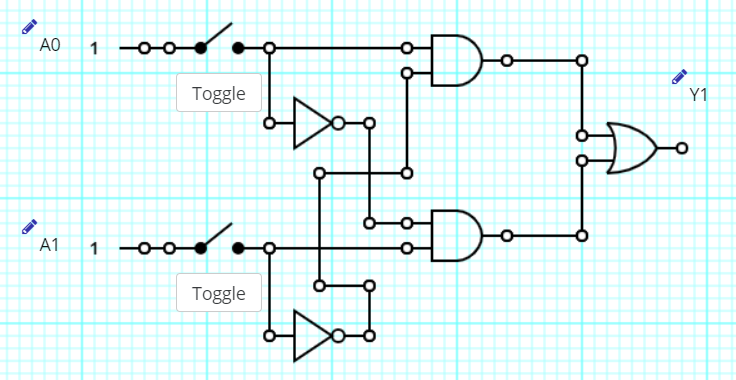
\includegraphics[width=\linewidth]{Y1CompuertasLogicas.png}
\end{figure}

\begin{figure}[htb] 
  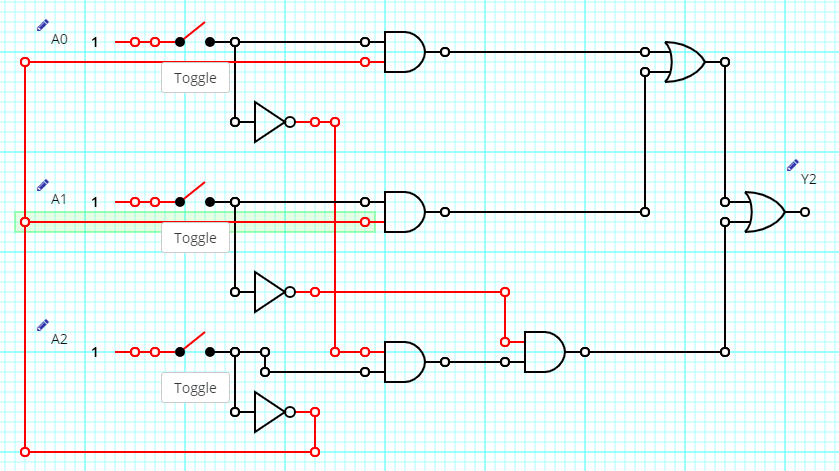
\includegraphics[width=\linewidth]{Y2CompuertasLogicas.png}
\end{figure}

\begin{figure}[htb] 
  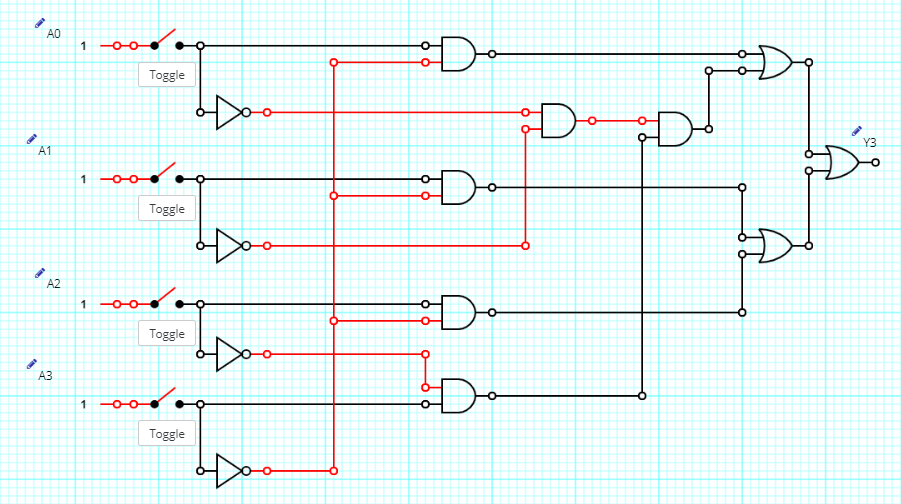
\includegraphics[width=\linewidth]{Y3CompuertasLogicas.png}
\end{figure}

\end{document}
